\begin{figure}
%  \begin{subfigure}[b]{.53\textwidth}
%    \centering
%    \begin{tikzpicture}
%
%      \node[inner sep=0pt] (img) at (0,0)
%           {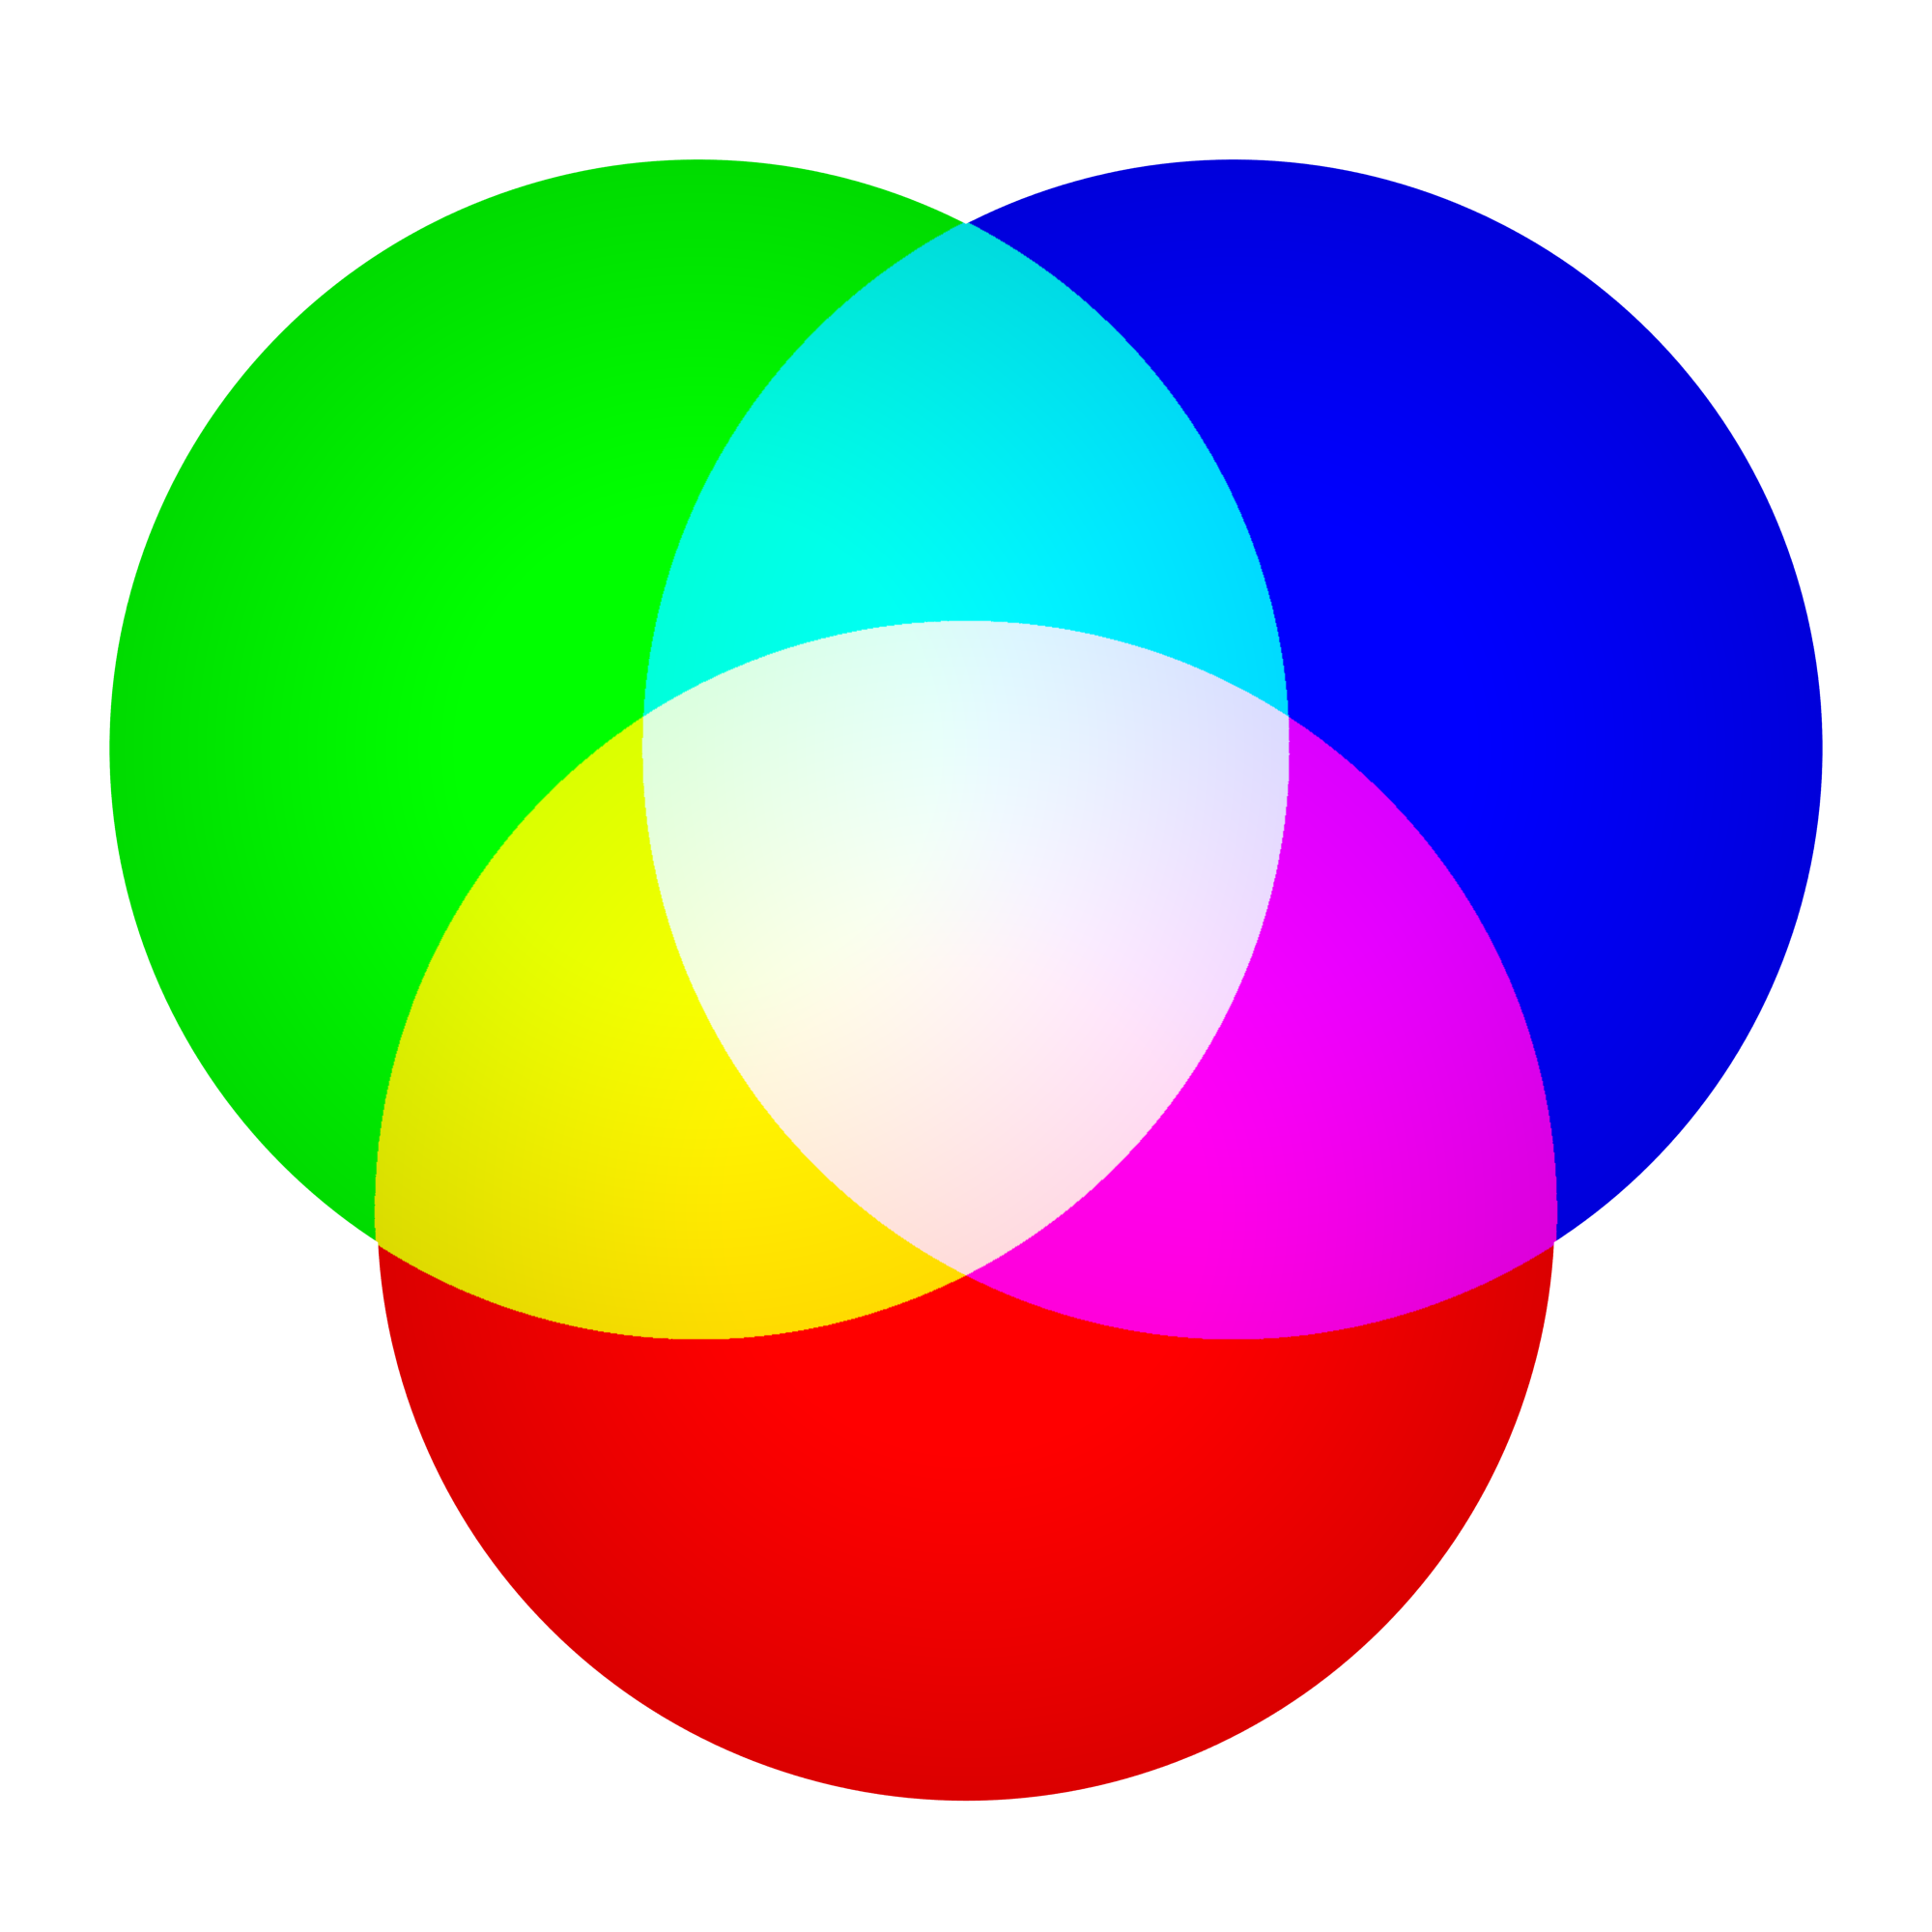
\includegraphics[width=\textwidth]{./img/raw/fw-kleur/colour-wheel1.png}};
%
%      \node (l1) at (0, 0) {Wit};
%      \node (l2) at (0, 1.8) {Cyaan};
%      \node (l3) at (-1.8, 1.3) {Groen};
%      \node (l4) at (1.8, 1.3) {Blauw};
%      \node (l5) at (-1.5, -0.5) {Geel};
%      \node (l6) at (1.5, -0.5) {Magenta};
%      \node (l7) at (0, -2) {Rood};
%    \end{tikzpicture}
%    \label{fig:fw-kleur:illustration}
%    \caption{Mengen van primaire kleuren.}
%  \end{subfigure} %
%  \begin{subfigure}[b]{.46\textwidth}
%    \centering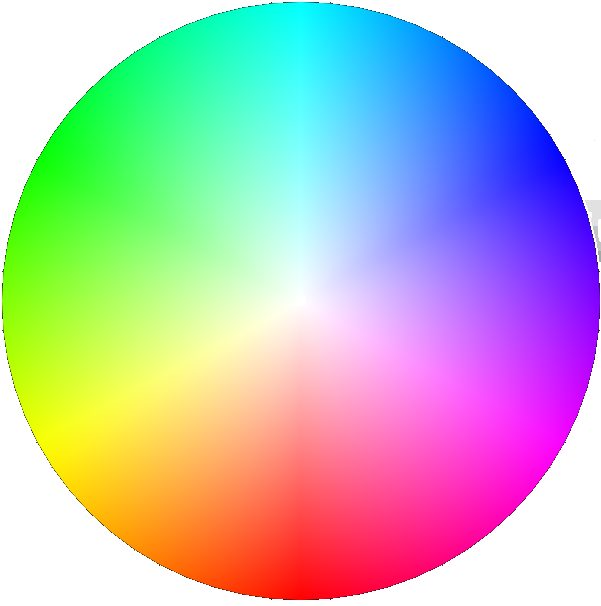
\includegraphics[width=0.4\textwidth]{./img/raw/fw-kleur/colour-wheel2.png}
%    \label{fig:fw-kleur:hsv}
%    \caption{Mengen van alle kleuren.}
  %  \end{subfigure} %
  \centering
\pgfdeclarefunctionalshading{HSVsweep}
{\pgfpoint{-2cm}{-2cm}}
{\pgfpoint{2cm}{2cm}}
{}
{ % x y
 2 copy % ... x y x y
 2 copy 0 eq exch 0 eq and
 { pop pop 0.0 } % silently deal with error: return
               % arbitrary heading of zero for origin
 {atan 360.0 div} % ... x y heading;  heading being in
                 %the interval [0, 1.0]
 ifelse  % because we will use it for 'Hue'
 dup 360 eq { pop 0.0 }{} ifelse % if heading is 360
                                 %degrees, make it zero instead
 3 1 roll % ... heading x y
 dup mul % ... heading x y*y
 exch dup mul % ... heading y*y x*x
 add sqrt % ... heading ra_pt (distance from origin in points)
 56 div % scale it means a ra of just under 2 cm
 dup 1.0 ge % BOOLEAN. ready to clamp to interval [0, 1.0]
 { pop 1.0 }{} ifelse % We shall use the scaled ra as 'Saturation'
 2.5 mul 0.25 sub % now, Ra in [0.1, 0.5] --> Saturation
                % in [0.0, 1.0]. Saturation varies between the two radii
 1 % ... H S V ( with 'Value' set to literal constant of 1.0 )
 1 index 1.0 eq % TEST I [ S == 1.0 ]
 { % BLOCK A [ take stack to V V V ] achromatic case
   3 1 roll pop pop dup dup
 }
 { % BLOCK B take stack to V T Q P i
   % C version to use as model:
     % H' = H * 6
     % i = floor(H')
     % f = H' - i
     % P = V * (1.0 - S)
     % Q = V * (1.0 - (S*f))
     % T = V * (1.0 - (S * (1.0 - f)))
   3 -1 roll 6.0 mul dup 4 1 roll % H' S V H'
   floor % H' S V i
   dup  5 1 roll % i H' S V i
   3 index sub neg % i H' S V f
   1.0 3 index sub % i H' S V f (1.0 - S )
   2 index mul % i H' S V f P
   6 1 roll % P i H' S V f
   dup 3 index mul neg 1.0 add % P i H' S V f ( 1.0 - (f*S))
   2 index mul % P i H' S V f Q
   7 1 roll % Q P i H' S V f
   neg 1.0 add % Q P i H' S V (1.0 - f)
   2 index mul neg 1.0  add % Q P i H' S V (1.0 - S * (1.0 - f))
   1 index mul % Q P i H' S V T
   7 2 roll % V T Q P i H' S
   pop pop % V T Q P i
   %%%
   % end of BLOCK B. The rest is just stack manipulation
   dup 0 eq % TEST II [ i == 0 ]
   { % BLOCK C [ take stack to V T P ]
   pop exch pop
   }
   { dup 1 eq % TEST III [ i == 1 ]
     { % BLOCK D [ take stack to Q V P ]
   pop exch 4 1 roll exch pop
     }
     { dup 2 eq % TEST IV [ i == 2 ]
       { % BLOCK E [ take stack to P V T ]
       pop 4 1 roll pop
       }
       { dup 3 eq % TEST V [ i == 3 ]
         { % BLOCK F [ take stack to P Q V ]
         pop exch 4 2 roll pop
         }
         { dup 4 eq % TEST VI [ i == 4 ]
           { % BLOCK G [ take stack to T P V ]
           pop exch pop 3 -1 roll
           }
           { % BLOCK H [ take stack to V P Q ]
           pop 3 1 roll exch pop
           }
           ifelse
         }
         ifelse % for V
       }
       ifelse % for IV
     }
     ifelse % for III
   }
   ifelse % for II
   % BLOCK I
 }
 ifelse % for I
 % BLOCK J
 % .. RGB at last
 % Fix for Apple's PDF viewer shading bug:
 cvr 3 1 roll cvr 3 1 roll cvr 3 1 roll 
}

  \begin{adjustbox}{minipage=\textwidth, scale=0.55}
  \centering
  \begin{tikzpicture}
    \def\ra{3.8cm}
    \def\raB{1cm}
    \draw[shading=HSVsweep,even odd rule] (0,0) circle (\ra) circle (\raB);
    \draw[fill=red] (-0+90:3.8) circle (0.5);
    \draw[fill=green] (-120+90:3.8) circle (0.5);
    \draw[fill=blue] (-240+90:3.8) circle (0.5);
  \end{tikzpicture}
  \end{adjustbox}
  \caption{Het mengen van kleuren volgens een additief model.}
  \label{fig:fw-kleur}
\end{figure}
